\documentclass[english,dit,thesis]{hogentreport}
\graphicspath{{img/}{graphics/}}

%% For source code highlighting, requires pygments to be installed
%% Compile with the -shell-escape flag!
%% Titelpagina
\usepackage{hogent-titlepage-image}

\usepackage[section]{minted}
\usemintedstyle{solarized-light}
\definecolor{bg}{RGB}{253,246,227} %% Set the background color of the codeframe
%% Change this line to edit the line numbering style:
\renewcommand{\theFancyVerbLine}{\ttfamily\scriptsize\arabic{FancyVerbLine}}

%% Macro definition to load external java source files with \javacode{filename}:
\newmintedfile[javacode]{java}{
    bgcolor=bg,
    fontfamily=tt,
    linenos=true,
    numberblanklines=true,
    numbersep=5pt,
    gobble=0,
    framesep=2mm,
    funcnamehighlighting=true,
    tabsize=4,
    obeytabs=false,
    breaklines=true,
    mathescape=false
    samepage=false,
    showspaces=false,
    showtabs =false,
    texcl=false,
}

%% Settings:
\author{Tom Antjon}
\title{Content~\\Management~\\Systems}
\academicyear{\advance\year by -1 \the\year--\advance\year by 1 \the\year}
\partialthesis{false} %% To display 'in partial fulfilment'
%\institution{Internshipcompany BVBA.}

%% Add global exceptions to the hyphenation here
\hyphenation{back-slash}

%% The bibliography (style and settings are  found in hogentthesis.cls)
\addbibresource{bibliography.bib}        %% Biblatex bibliography file
\defbibheading{bibempty}{}

%% Prevent empty pages for right-handed chapter starts in twoside mode
\renewcommand{\cleardoublepage}{\clearpage}

\renewcommand{\arraystretch}{1.2}

%% Content starts here.
\begin{document}

    \inserttitlepage{achtergrond-ozt.png}

%-----------------------------------------------------------------------------
% Copyright
%-----------------------------------------------------------------------------

\newpage

\thispagestyle{empty}

\vspace*{20cm}

\noindent Copyright \copyright\ 2023-{\the\year} Tom Antjon % Copyright notice

\noindent \textsc{www.hogent.be} % URL

\noindent \textit{Gegenereerd op \today} % Printing/edition date

%-----------------------------------------------------------------------------
% Inhoudstafel
%-----------------------------------------------------------------------------

\usechapterimagefalse
\tableofcontents % Print the table of contents itself

\cleardoublepage % Forces the first chapter to start on an odd page so it's on the right

\def\R{\mathbb{R}}

%-----------------------------------------------------------------------------
% Corpus
%-----------------------------------------------------------------------------

\chapter{Introduction}
\label{ch:introduction}

E-commerce has been around for a number of decades by now. Since the release of the Netscape browser in 1994 companies have been selling their products online. From 1995 to 2000 the number of companies who were selling their products online increased significantly. Venture capitalists invested huge amounts of money in these new internet companies. Sadly, the excitement wasn’t well founded. The world wasn’t ready for a shift from traditional retailing to e-commerce. People were wary about ordering products online, online payment methods weren’t very widely accepted and parcel services weren’t optimized for delivering the products to the people.

The excitement about internet companies led to the dotcom bubble bursting in 2000. A lot of new internet companies went bankrupt, others had to downsize significantly. A lot of survivors of the dotcom bubble are still around today. They have now become huge internet companies, some examples are: amazon.com, ebay.com and dell.com.

In the last 15 years online retailing has been steadily increasing. People were getting more comfortable buying their products online, online payment methods improved significantly and parcel services optimized their distribution network. These improvements gave small companies the opportunity to start selling their products online.
The speed at which ecommerce is cutting into traditional retail’s market share is incredible. Q1 2010 saw just 4.2\% of US retail sales happening online. In Q1 2019 that was 10.5\%. The pandemic and subsequent lock-downs took that to 16.1\% in Q2 2020.

It’s worth noting that the pandemic has accelerated consumer adoption of e-commerce, and this growth looks to be exponential. It’s expected that 95\% of the global retail market will be happening online by 2040. \cite{RetailVsEcom2022}

\section{Course content}
In this course you will learn to create and manage a web store. There are a lot of platforms which allow you to create a web store. In this course we chose to use Drupal. Drupal is a content management system (CMS) written in PHP. It has many features that will make it easy to create a web store.

First we’ll learn how to create, manage and edit a basic Drupal site. Afterwards we’ll add the web store functionality through the use of modules. During the course you’ll also learn how to write PHP code, manage your site through git, collaborate on your site and deploy it to a server.

\section{What is a CMS?}
Drupal is a content management system or CMS. The name is a good description of what it actually does. It’s an application which makes it easy to manage content. The content can be of different types. For example, a blog can use a CMS. The type of content on the blog will be articles. The CMS makes it easy to create, edit, remove and manage articles. Another example where a CMS can be useful is when you create a web store. The type of content we use here are products. The CMS makes it easy to manage the products, for example: add a product, change the price or add a shipping method.
A lot of big websites use a CMS as their background application. Examples include: www.engadget.com, www.puma.com, www.societegenerale.com. Figure \ref{fig:cms_systems} shows different CMS systems.

\begin{figure}[h]
    \centering
    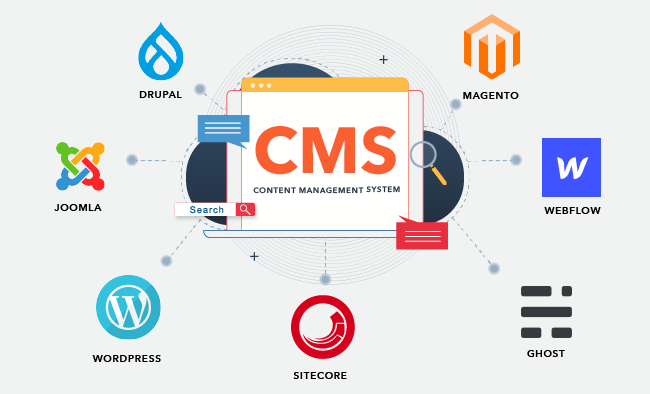
\includegraphics[width=1\linewidth]{img/ch1/cms_systems}
    \caption{A lot of different CMS systems are available on the market, Drupal being one of them \cite{HubSpot2022}}
    \label{fig:cms_systems}
\end{figure}



\section{What is Drupal?}
As mentioned before, Drupal is an open source CMS written in PHP. Drupal is web based so it uses HTML, CSS and JavaScript as application front end. A Drupal application is completely customizable. We can change the look of our site by changing the HTML and CSS (Drupal calls this theming).
The application back end can be extended by adding our own code or code other people made available online (Drupal does this through its module system).
Drupal was created in 2001 by Dries Buytaert. He got his degree in computer science at the university of Antwerp and his PhD at Ghent university. In 2007 he started the company Acquia which provides services to organizations using Drupal as their CMS. In 2009 Acquia helped with the relaunch of Whitehouse.gov. Next to whitehouse.gov a lot of other sites use Drupal. At https://www.drupal.com/showcases you can find a list of different sites build with Drupal.

\subsection{Drupal 10}
Drupal 10 was released in December, 2022, which continues to build on the same base as Drupal 8. The release of Drupal 8 was a major milestone, giving life to a new Drupal. The codebase was completely reworked and a now roadmap was drawn. Development continued to build on this new code base with the latest version being 10.1.

\section{Review Exercise}
\begin{enumerate}
    \item Look up the definition of a CMS on Wikipedia.
    \item Think of five content types that could be managed by a CMS.
    \item Find five sites which use Drupal as CMS.
    \item Name three other content management systems.
\end{enumerate}

\chapter{Installation}
\label{ch:Installation}

To run a Drupal website, 3 things are needed:
\begin{itemize}
    \item A WebServer, i.e. Apache
    \item A Database, i.e. MariaDB, MySQL, SQLite...
    \item A PHP Runtime Environment
    
\end{itemize}


These requirements can be hosted online via AWS, Combell, Pantheon.io... or you can set up a local development environment via an AMP stack. Depending on your operating system, there are multiple options. On Windows, XAMPP can provide this development environment, but you can also use Docker to containerize and set up a Lando Development Environment.

Whatever environment you choose, it is always recommended to manage your Drupal website via composer. In the following sections, we'll setup a XAMPP environment and install all necessary tools to get started. We'll also reference some options.

\section{XAMPP}
\label{sc:xampp}
When we want to download XAMPP\footnote{https://www.apachefriends.org/download.html}, there are different versions, linked to the PHP version that is included. Depending on the Drupal Version you want to install, you need to have PHP version support. Always check the release notes or official documentation to know the right Drupal version requirement. Drupal version 10.1 needs PHP version 8.1 or higher\footnote{https://www.drupal.org/docs/getting-started/system-requirements/php-requirements}.

On the moment of writing, PHP version 8.2.4 is the latest version supported by XAMPP, so that would be the best choice to be future-proof as well. If you want to host an older version of Drupal or have a legacy site to maintain, be sure to have the right environment.

Once XAMPP is installed, run the application and make sure Apache and MySQL are up and running.

\begin{figure}[h]
    \centering
    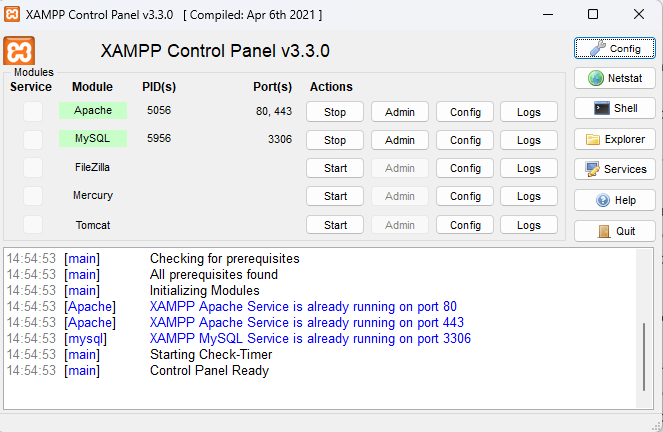
\includegraphics[width=1\linewidth]{img/ch2/xampp}
    \caption{XAMPP Control Center}
    \label{fig:xampp}
\end{figure}

To make sure we can install Drupal and run it smoothly, we need to change some configuration for Apache and MySQL. This can be done using the Config buttons in the XAMPP Control Panel for each service.

First we need to enable the PHP Extension GD. Go to the PHP.ini file via the Apache Config and remove the semi-colon that comments out the extension gd.

\begin{minted}{bash}
    extension=gd
\end{minted}

Be sure to re-start Apache once the settings have been changed.

\section{Composer}
Composer is an application-level package manager for the PHP programming language that provides a standard format for managing dependencies of PHP software and required libraries. 
It is the most recommended tool to install Drupal.
It will be used during the course to install, extend and manage Drupal.

Composer can be installed on all operation systems, it only needs a PHP installation.
In our case we've installed PHP by installing XAMPP in \ref{sc:xampp}.

    Detailed instructions to download and install composer can be found on the official website\footnote{https://getcomposer.org/download/}


\section{Other options}
As mentioned before, there are a number of other options that can be used to host Drupal Websites. Below we'll highlight a few which might be useful to look at.
\subsection{Pantheon.io}
Taken from the Pantheon website\footnote{https://pantheon.io/}:

\begin{quote}
Pantheon is the single SaaS platform provider that affordably integrates website development, management, performance, team education and hands-on account support. All with enterprise-grade security and the world's fastest hosting. All in one secure environment.
\end{quote}

Especially when working with a team, it can be interesting to host your Drupal website on Pantheon. You can all share the same development environment and the code is stored in a GIT repository which can be cloned and ran locally as well.

Open a free account and create a new Drupal 10 website with an easy wizard.

\subsection{Combell}
Combell is a webhosting company where you can host your own website and provides domainname registration as well.

Via AcademicSoftware\footnote{https://www.academicsoftware.eu/}, a student of Hogeschool Gent can request free hosting, which also includes a domainname. 

Several packages are possible, but for Drupal make sure to take the Combell Web Hosting (Linux) package. 

Once acquired, you can create up to 4 websites on that hosting. You can access the hosting via SFTP or SSH, or use the one-click install to launch a CMS like Drupal, Wordpress or Joomla.


\subsection{Docker Bases development environments}
As a final noteworthy mention there are Docker-bases development environments like DDev\footnote{https://ddev.com/} and Lando\footnote{https://lando.dev/}. A one-stop shop for creating a dev environment using a Docker engine backend and can run on Windows, MacOS and Linux.

For Windows the WSL2 feature needs to be enables. You can find all the details on the documentation websites of DDev or Lando.







\chapter{Creating a Drupal Site}
\label{ch:creating_a_drupal_site}

Moving forward in this course, we'll be using XAMPP on Windows. We'll create and manage our websites the recommended way, using composer.

\section{Create a new Drupal site using composer}
To install a new Drupal site using composer is very easy and only requires one command:

\begin{minted}{bash}
    composer create-project drupal/recommended-project my_site_name_dir
\end{minted}

This will download the latest stable version\footnote{Make sure that your environment meets all the requirements of the Drupal Version. For Drupal 11, PHP 8.3 is necessary as well as a certain version of MySQL. XAMPP does not always support the latest version of PHP/MySQL. You can install other versions of Drupal by defining the version in composer i.e. drupal/recommended-version:10.3.5} of Drupal in the current folder. WHen using XAMPP, you need to put all your websites in the htdocs folder of your XAMPP installation. The default path would be 'C:\textbackslash xampp\textbackslash htdocs'.
\\\\
The 'recommended-project' creates Drupal the recommended way:
\begin{itemize}
    \item All the Drupal files are located in the web folder
    \item All the external modules/libraries are held separately in the vendor folder
    \item Composer.json file is created
    \subitem Holds reference to the installed dependencies
    \item	Composer.lock file is created
    \subitem Holds reference to the exact versions of the installed dependencies
   \item Gitignore 
\end{itemize}

\section{Create a new database}
If we want to install a new Drupal website, we also need a database to store our data. When going through the installation process, Drupal will ask us for the connection details to the database.

We can create a database using phpMyAdmin in XAMPP. Or if you have a MySQL server running locally, you can use other tools like MySQL Workbench.

Using phpMyAdmin\footnote{http://localhost/phpmyadmin/}, you can create a new website using the GUI, see figure  \ref{fig:db_create}. Let's create a new database called drupal\textunderscore newssite.


\begin{figure}[h]
    \centering
    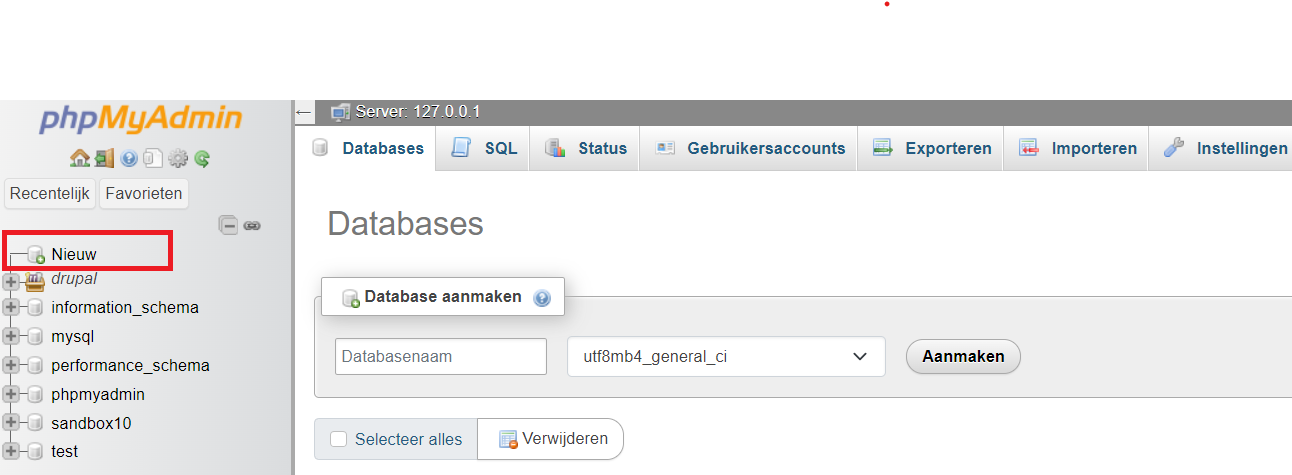
\includegraphics[width=1\linewidth]{img/ch3/createDB}
    \caption{You can manage your databases via phpMyAdmin}
    \label{fig:db_create}
\end{figure}

\section{Install Drupal}
Now that everything is in place, we can browse to our new website and start the installation process.

Using XAMPP, you can find your websites by navigating to https://localhost/<site-folder>. For example, if we use composer to create a new website in de htdocs folder, with the name newssite, we can browse to https://localhost/newssite.

From here, we can navigate to the web folder, which holds our index.php file and is our entry point to the website.

Now we are shown the installation screen where we need to select the language to install Drupal in. We'll choose 'English' and click 'Save and continue'.

\begin{figure}[h]
    \centering
    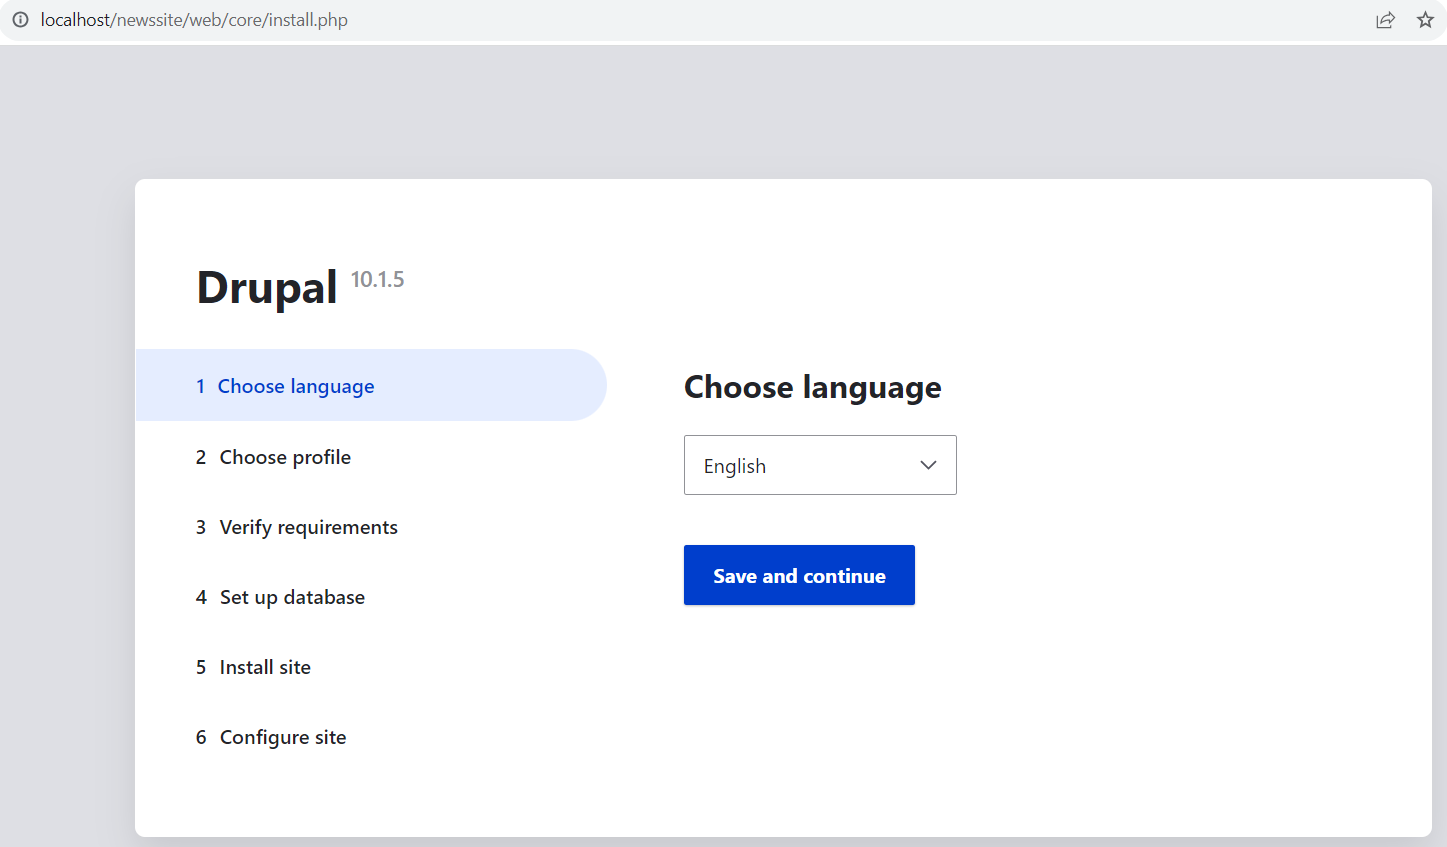
\includegraphics[width=1\linewidth]{img/ch3/install_step1}
    \caption{Follow the installation wizard to install a fresh Drupal website}
    \label{fig:install_step1}
\end{figure}

Next we'll stick with the standard installation and in step 3 Drupal shows us the requirements to continue the installation. We can ignore warnings, but errors need to be fixed. Drupal always provides information what's wrong, and how to fix it. At the bottom of the page we can click 'continue anyways' to ignore the warnings and continue the installation.

\begin{figure}[h]
    \centering
    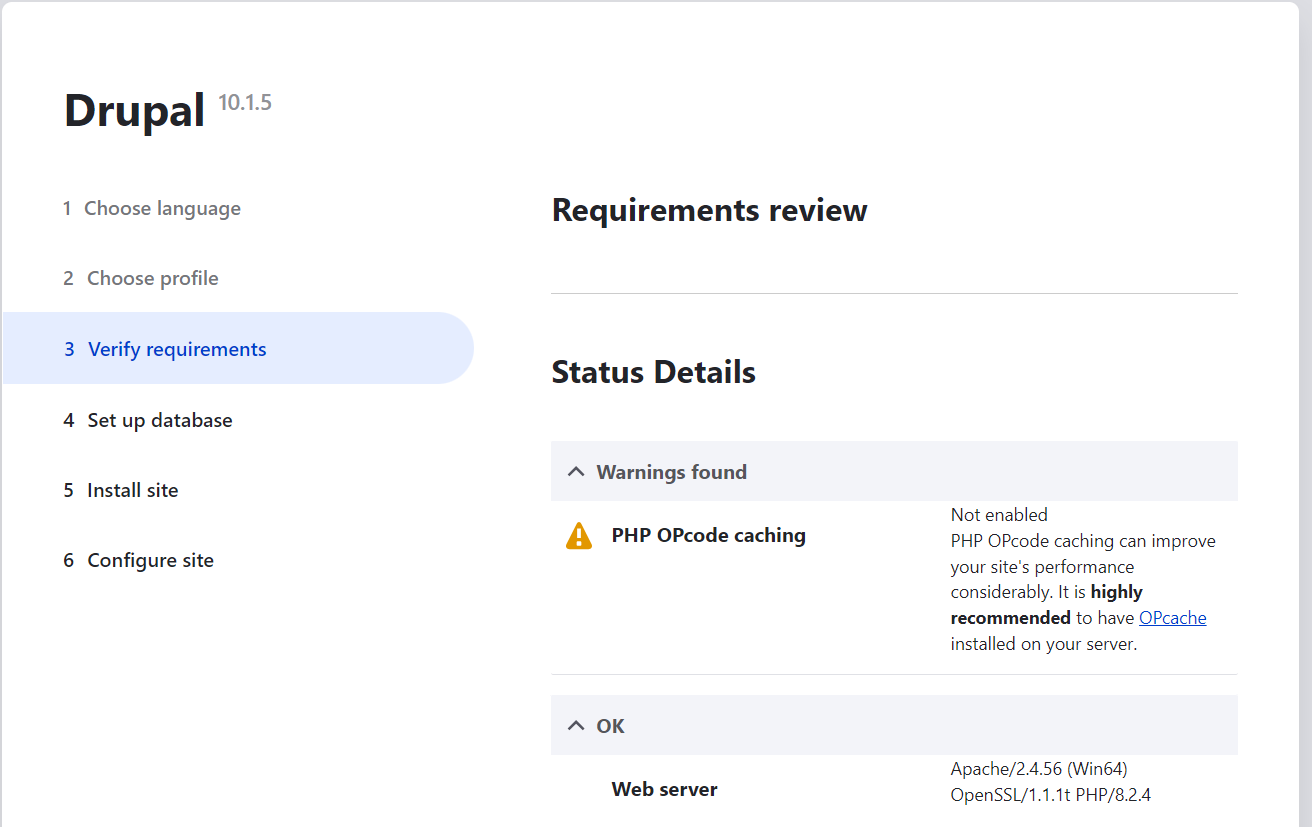
\includegraphics[width=1\linewidth]{img/ch3/install_step3}
    \caption{An overview of the minimum requirements to install Drupal}
    \label{fig:install_step3}
\end{figure}

In step 4, we need to enter the details of the database we created earlier. In our example, the database name is 'drupal\textunderscore newssite'. The database username and password depend on your installation. The default is set to 'root' as username without any password. But this can differ from your set up. If your database is running on a different server and or port, you can change it in the advanced options section.

\begin{figure}[h]
    \centering
    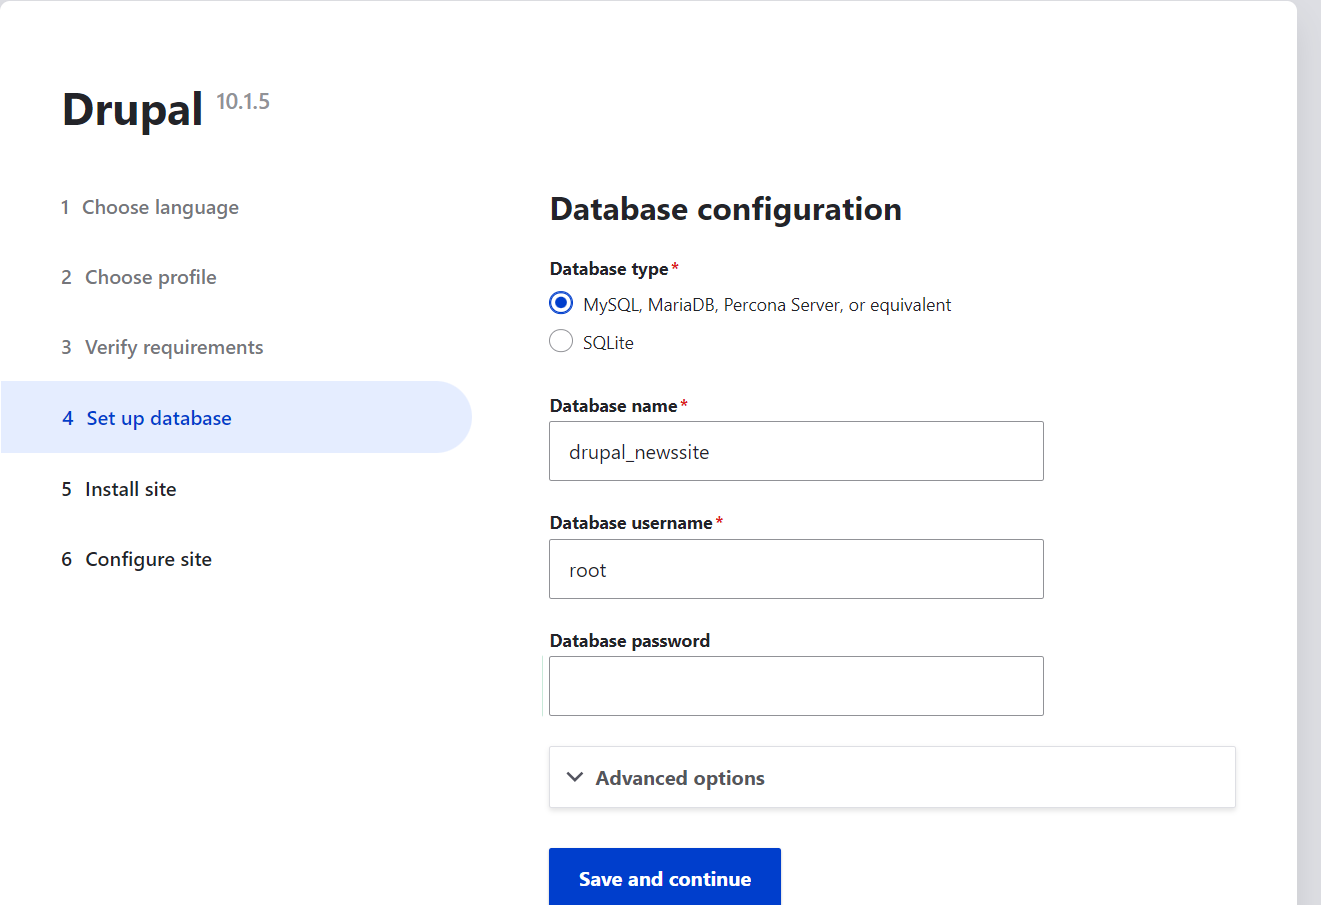
\includegraphics[width=1\linewidth]{img/ch3/install_step4}
    \caption{Setup the connection to the database}
    \label{fig:install_step4}
\end{figure}

Drupal continues to install the website and connect to the database to store all necessary data. In step 6, we finish up by entering some website details. These can be changed later in the administration tools as well.

\begin{figure}[h]
    \centering
    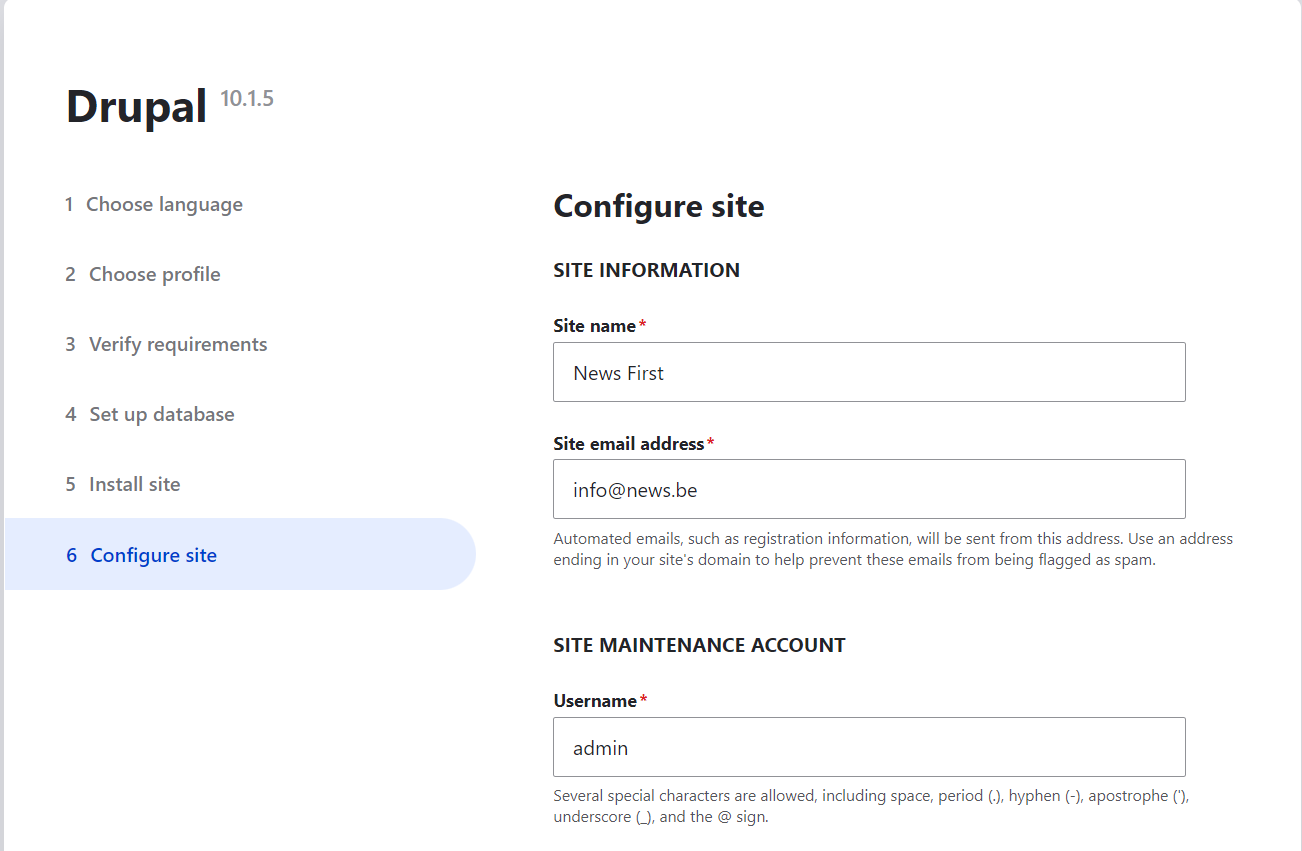
\includegraphics[width=1\linewidth]{img/ch3/install_step6}
    \caption{Enter the site details}
    \label{fig:install_step6}
\end{figure}

For our site we'll fill in the following details:
\begin{itemize}
    \item Site name: Newssite
    \item Site email address: info@news.be
    \item Username: admin
    \item Password: drupal
    \item Select your regional settings
    \item Untick the box 'Receive email notifications'. Seeing this is a sample site, this is not necessary.
\end{itemize}


\begin{figure}[h]
    \centering
    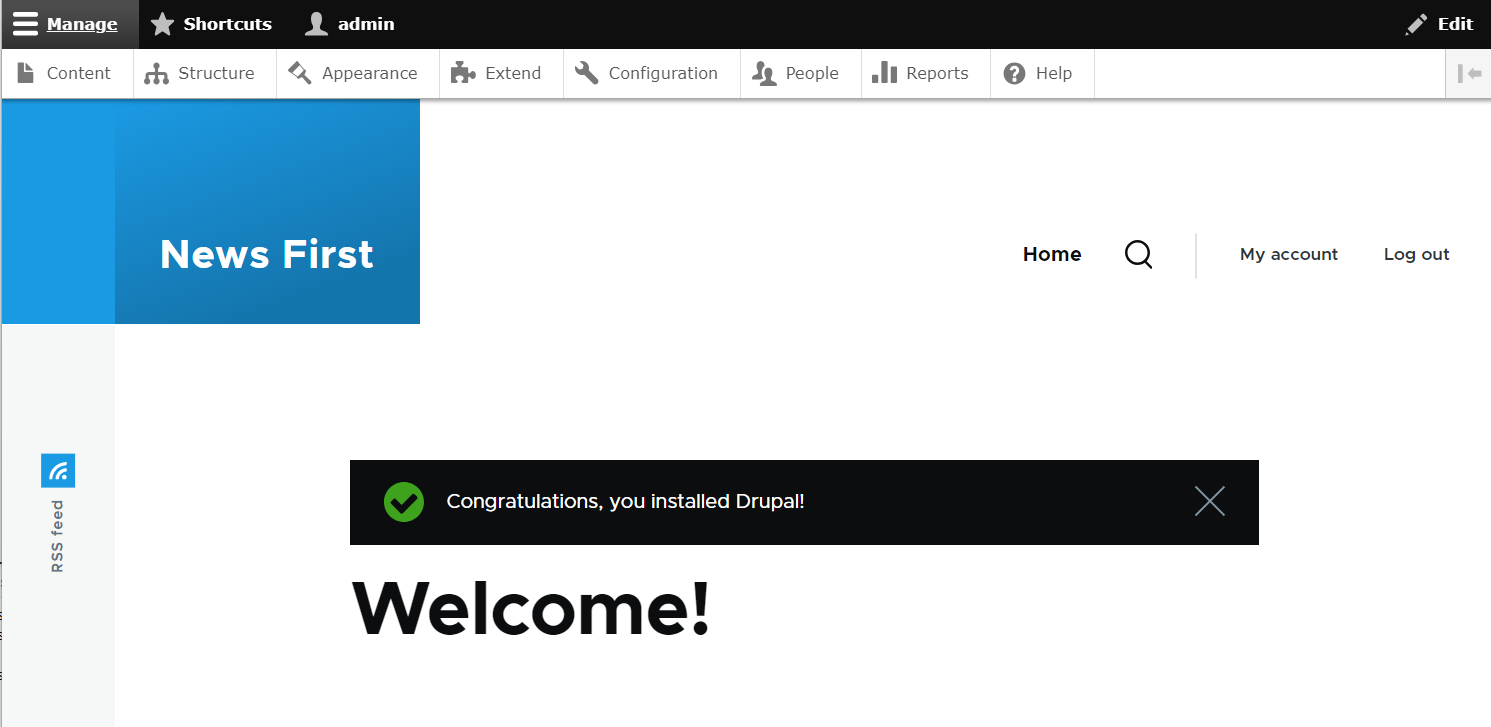
\includegraphics[width=1\linewidth]{img/ch3/install_complete}
    \caption{A fresh Drupal website}
    \label{fig:install_complete}
\end{figure}

Et voila, you have your first Drupal site. It’s pretty basic, you only have a welcome page, no content yet. By default, after completing the installation, you are logged in as administrator. To see the non-administrator layout, click the Log out link in the top right corner. As you can see, we only have a basic one-page site with our site title at the top. Now log back into your site with username: admin and password: drupal.

\section{Review exercise}

Create a new Drupal site with the following properties:
\begin{itemize}
    \item Site name: bitingbugsexample
    \item Site email address: noreply@bitingbugsexample.com
    \item Username: admin
    \item Password: drupal
    \item Email address: info@bitingbugsexample.com
    \item Default country: Belgium
    \item Default time zone: Europe/Brussels  
\end{itemize}








\chapter{Drupal Structure}
\label{ch:drupal_structure}

\section{Core concept}
Drupal uses entities. The concept of entities is in reality a pretty complicated one, but mostly to developers. This is because Drupal’s API contains some nifty functionality concerning Entities, but to most webmasters, site builders and themers alike, Entities don’t have to be that complicated. 
Entities are like furniture, for example a bookshelf. By itself, a bookshelf doesn’t do very much. It’s actually not that interesting, it just IS. But add some books, change the shelving, mix it up a bit and add some pictures, and the bookshelf becomes a design centre piece of your living room.... Now imagine you could reuse those pictures in different sizes or frames... all over your living room! You could definitely throw together some interesting compositions! 
\subsection{Fields} 
All of the entities in Drupal are ‘fieldable’, meaning we can add fields to them. A field is a reusable piece of content. A field has a primitive data type like Boolean or Decimal or Text or Image or file etc. With the help of fields we define custom content types, taxonomies etc.... 

\subsubsection{Field Types} 
General: 
\begin{itemize}
    \item Boolean ­ On/off checkbox 
    \item Comments ­ This field adds a ‘Add comment’ form and the submitted comments 
    \item Date 
    \item E­mail 
    \item Link 
\end{itemize}

Number: 
\begin{itemize}  
    \item List (float) ­ A list of numeric values. 
    \item List (integer) ­ A list of numeric values. 
    \item Number (decimal) 
    \item Number (float) 
    \item Number (integer) 
\end{itemize}

Reference: 
In Drupal we can link pieces of content to each other by using a reference field, referenced items can be partially or fully displayed if you want to. All the following entities can be referenced: 
\begin{itemize}  
    \item Content 
    \item File 
    \item Image 
    \item Taxonomy term 
    \item User 
    \item Other 
\end{itemize}

Text:
\begin{itemize}
    \item Text (formatted) ­ A single line text field, for short texts, allows formatted text (like html or wysiwyg). 
    \item List (text) ­ A list of text values. 
    \item Text (formatted, long) ­ A text area with multiple rows, allows formatted text (like html or wysiwyg). 
    \item Text (formatted, long, with summary) ­ Same as above but with an extra text area to add a summary. 
    \item Text (plain) ­ A single line text field, for plain unformatted text. 
    \item Text (plain, long) ­ A text area with multiple rows, for plain unformatted text. 
\end{itemize}


\section{Structural elements}
Drupal core defines eight types of structural elements. To see an overview of those elements click on the Structure button in the administrative menu

Figure 4.1: Structural Elements

Each of these elements has a certain use within Drupal. The following list describes each of the structural elements. Don’t worry if not all the elements are clear to you, when you start changing and using your site the structure will become clear.

\textbf{Block layout}: Blocks are site elements which can be positioned in different places on your site. For example, the search field, which is visible on the left side of your first Drupal page, is a Drupal block. You can put a block in different places on your page, these places are called regions. These regions depend on the Drupal theme you are using. When you click the Block layout link you will see the following page (Figure 4.2).

Figure 4.2: Block layout

This page shows a list of the different regions and allows you to add blocks to each of these regions. You can click the link Demonstrate block regions(Bartik) to view the regions of the current theme (Bartik) (Figure 4.3).

Figure 4.3: Bartik regions

\textbf{Comment types}: The comment types page allows you to create and manage different comment types. When you add content to your site you can allow people to comment on the new content. The comment type defines the fields that the commenter has to fill out when he’s writing his comment. The default comment type has only one field: the comment body. We could, for example, create a new comment type which includes a field for the name and age of the commenter.
Contact form: The Personal contact form is the form for site visitors to contact registered users; the name and recipients of this form cannot be edited. Other forms listed here are your configured site-wide contact forms, which site visitors can use to send mail to a centralized email address or addresses. You can edit the name and recipients of site-wide forms by choosing the Edit operation. You can also configure the fields and display of both personal and site-wide forms.
Content types: The content types page is very important. The content types define which kind of information your CMS will manage. A content type has different fields. These fields define the information that is stored in the content type. By default, Drupal has two content types: Article and Basic page (Figure 4.4);

Figure 4.4: Default content types

When you click the Manage fields button on the right you can see what kind of information is stored in this content type. (Figure 4.5). As you can see, the Article content type has four fields: Body, Comments, Image and Tags.

Figure 4.5: Article content type fields

Next to the Manage fields menu item tab you have the Manage form display and Manage display tabs. These allow you to edit which fields are displayed when an element is created/edited or viewed.

\textbf{Display modes}: Display modes define different ways in which information is displayed. There are two types of display modes: form modes and view modes. Form modes are used when the content is created or edited, view modes when the content is viewed. When you go to Display modes → View modes (Figure 4.6) you will see the different ways in which a content type can be displayed.

Figure 4.6: Default view modes
When you go to Structure → Content types → Article → Manage display you will see the following page:

Figure 4.7: Display modes
There you see the different display modes that you can use for your Article content type. At the bottom of the page you can enable other display modes in the custom display settings dropdown (Figure 4.8).

Figure 4.8: Custom display settings
\textbf{Menus}: Menus are easy. They define a menu with different menu items. Each menu has a corresponding block that is managed on the Block layout page.
\textbf{Taxonomy}: A taxonomy defines lists of terms. These terms can be associated with the content. A list of terms is called a vocabulary. For example: if we have a site with news articles about sports we could add a tag to each article to tell what the article is about. These tags can be defined in a vocabulary.
\textbf{Views}: A view enables you to create a display based on different content types. This course has a whole chapter dedicated to Drupal Views so we won’t go into details here.
\section{Our example}
\subsection{Change the site title and logo}
To make our site a little bit prettier we will change the logo and title. To change the site title, go to Configuration → System → Basic Site settings. Change the site name there to Our first Drupal 8 site (Figure 4.9).

Figure 4.9: Changing the site title
The logo is part of the Drupal theme you are using. To change the logo, go to: Appearance → Settings → Bartik → LOGO IMAGE. Uncheck Use the default logo supplied by the theme and upload the file drupal\textunderscore 8 \textunderscore logo.png (Available in the course files zip). Click Save configuration.

Figure 4.10: Changed logo and title
4.2.2	Removing the Search and Tools block
On the right side of the page we have the Search and Tools block. We don’t need them for now so you can remove them by going to Structure → Block layout and disable  them (Figure 4.11). Click Save blocks.

Figure 4.11: Disable an existing block 
\subsection{Adding a Taxonomy}
To categorize the new items on our site we will add a taxonomy. This taxonomy will contain different types of news. Go to Structure → Taxonomy → Add vocabulary. Use the following settings:
Name: news categories
Description: Describes the type of the news item.
Click Save. In Figure 4.12 you can see the empty vocabulary. Next we will add some terms to the vocabulary. 
Figure 4.12: Adding vocabulary terms
Click the Add term button and add the following terms:
\begin{itemize}
    \item national news
    \item international news
    \item sports 
    \item media
\end{itemize}


Figure 4.13: Adding a vocabulary term
To see an overview of the terms you have added go to Structure → Taxonomy and click the List items button next to your vocabulary. (Figure 4.14)

Figure 4.14: Vocabulary terms
\subsection{Adding the News Item content type}
Since we are going to store news items in our CMS we will need to add the News Item content type. Go to: Structure → Content types → Add content type.
Give it the following properties:
Name: News Item
Description: Some news!
At the bottom of the page you can see some settings for this content type. Explore the settings, the names are very descriptive so most of them should be clear without further explanation. These are general settings that apply to all instances of this content type. You are able to change these for each instance individually when you create them.
Click Save and manage fields.

Figure 4.15: Manage fields
Add the following fields to the News Item content type: 
Body: (this item is already there, leave it as it is)
NewsTitle: (Text/plain, Maximum length = 255, number of values = 1) 
Image: (Image, number of values = 1)
News category: (Taxonomy term, number of values = unlimited, reference method = default, Vocabulary: news categories, Create referenced entities if they don’t already exist).
In figure 4.16 you can see an overview of the fields.

Figure 4.16: News item fields
\section{Review exercises}
In the following exercises we will review the content of this chapter by applying it to an example website. In the previous chapter we created the bitingbugs example website through the Acquia Dev Desktop. In this and the following chapters we will keep adding features to this site. Our goal is to create a web store for selling edible insects. The site will also provide a database with recipes so people know how to cook with the insects.

\begin{enumerate}
    \item Log in to your bitingbugs site (created in the previous chapter). Change the site name to Biting Bugs, and upload the file bitingbugs\textunderscore \textunderscore logo \textunderscore transp \textunderscore white\textunderscore right\textunderscore small.png (Available in the course files zip) as logo for the site, and bitingbugs-favicon.png as favicon.
    \item Add the search block to the sidebar second region and disable the powered by Drupal block.
    \item Add a comment type Answer to your bitingbugs site. We will use the comment type to allow users to answer a question. The comment type has two fields: answer (a number between 0 and 100000) and motivation (a textual explanation describing how they got the answer).
    \item\ Add vocabulary Food types type recipe to your bitingbugs site. Add the following terms to the vocabulary: Indian, Chinese, vegetarian, vegan, baking
    \item Add a new content type recipe to your bitingbugs site. The new content type has the following fields: Name (=Title), Ingredients (formatted, long), Directions (formatted, long, with summary), Plate image, Estimated time (integer, in minutes), Type (food types)
    Make sure the teaser only displays the Title and Image fields.
\end{enumerate}

\chapter{Creating Content}
\label{ch:creating_content}
\chapter{Users}
\label{ch:users}
\chapter{Views}
\label{ch:Views}
\chapter{Multilingual and Translations}
\label{ch:multilingual_translations}
\chapter{Drupal Theming}
\label{ch:drupal_theming}
\chapter{Collaborating on a Drupal Website}
\label{ch:collab}
\chapter{Drupal Commerce}
\label{ch:commerce}
\chapter{Introduction to PHP}
\label{ch:intro_php}
\chapter{Module building}
\label{ch:module_building}
\chapter{SEO in Drupal}
\label{ch:seo}


\begin{appendices}
    %\include{logistic}
    
    
    \clearpage
    \addcontentsline{toc}{chapter}{\textcolor{maincolor}{\IfLanguageName{dutch}{Bibliografie}{Bibliography}}}
    \printbibliography[heading=bibintoc]
    
    
    \clearpage
    \addcontentsline{toc}{chapter}{\textcolor{maincolor}{Index}}
    \printindex
    
\end{appendices}
\end{document}

